\section{결과 및 결론}

유전 알고리즘을 돌려본 결과, 아래의 그림과 같이 유전 알고리즘이 잘 수렴하였음을 확인할 수 있었으며, 그 결과의 분포 역시 시각화 가능하였다. 이를 통하여 유전 알고리즘의 결과가 실제 계산으로 도출된 결과와 얼마나 유사한 지를 정성적으로 확인 가능하다. 그리고 유전 알고리즘을 작동시키는 과정에서 선택압을 적절히 조절함으로써 해의 수렴성을 높일 수 있다는 사실도 알 수 있었다.

또한, 자체 제작한 평가함수를 이용한 유전 알고리즘의 결과가 KL 지표 상으로도 수렴하고 있음을 확인해볼 수 있는데, 이는 유전 알고리즘에 사용된 평가함수가 정확하였다는 것을 시사한다. 그리고 KL 값 자체가 0으로 수렴하였기 때문에 유전 알고리즘으로 도출된 분포가 통계적으로 실제 수식적으로 유도된 분포와 거의 같다는 것을 정량적으로도 확인해볼 수 있었다. 

다만, 아래의 (Fig. \ref{fig:normal fitness}.)에서는 다른 분포들의 시뮬레이션과는 다르게 KL의 수렴 그래프를 싣지 못하였는데, 이는 앞선 언급했듯이 정규분포의 식은 이산적인 상황에서 유도하지 못하였기 때문이다. 그러나 이 상황에서 역시 적합도 값은 잘 수렴한다는 사실을 알 수 있었다. 그리고 대안으로 같은 평균과 표주편차 값을 갖지만 $(-\infty, \infty)$를 정의역으로 갖는 실제 연속적인 정규 분포와의 대조해보았는데, 그래프의 개형이 거의 유사하다는 것을 알 수 있었다.

결론적으로 본 연구를 통해 정보 엔트로피의 최대화에 다양한 제약 조건을 입히는 것만으로도 우리가 잘 아는 균등 분포, 볼츠만 분포, 그리고 정규 분포가 잘 유도됨을 보일 수 있었다. 특히, 이 과정에서 라그랑주 승수법을 활용하여 다변수 함수의 최솟값을 찾을 수 있었으며, 유전 알고리즘을 통해 이가 실험적으로 검증해볼 수 있었다.

\pagebreak
\begin{figure}[!htb]
    \centering
    \begin{minipage}{.5\textwidth}
        \centering
        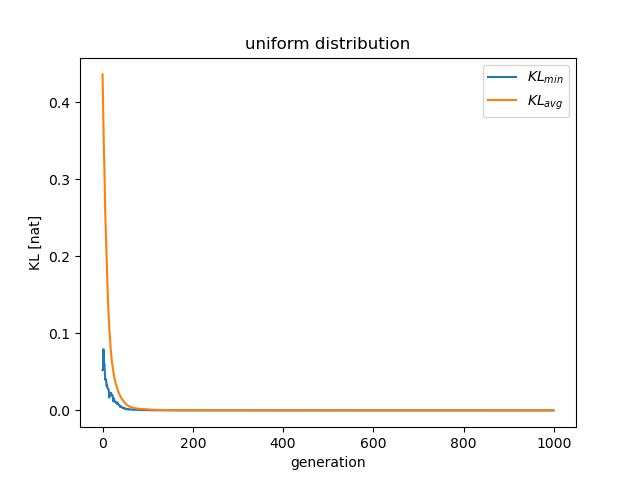
\includegraphics[width=\linewidth, height=0.63\linewidth]{images/uniform convergence KL.png}
        \caption{균등 분포의 KL 수렴 양상}
        \label{fig:uniform KL}
    \end{minipage}%
    \begin{minipage}{0.5\textwidth}
        \centering
        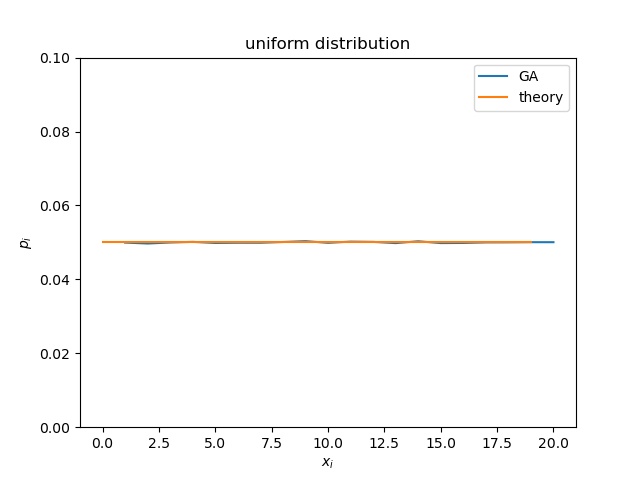
\includegraphics[width=\linewidth, height=0.63\linewidth]{images/uniform result.png}
        \caption{균등 분포의 수렴 결과}
        \label{fig:prob1_6_1}
    \end{minipage}
\end{figure}
\begin{figure}[!htb]
    \centering
    \begin{minipage}{.5\textwidth}
        \centering
        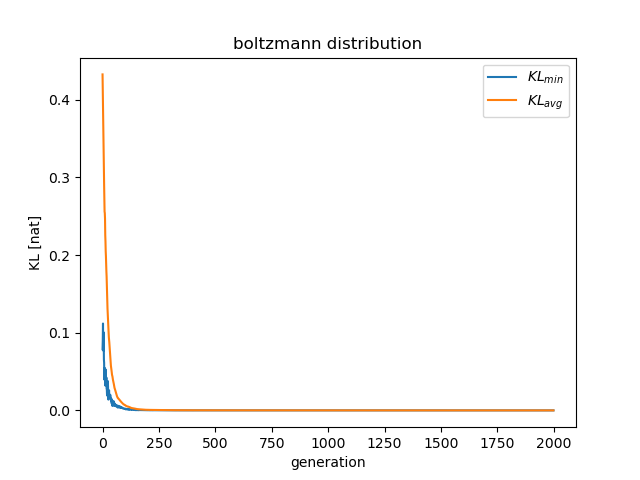
\includegraphics[width=\linewidth, height=0.63\linewidth]{images/boltzmann convergence KL.png}
        \caption{볼츠만 분포의 KL 수렴 양상}
        \label{fig:prob1_6_2}
    \end{minipage}%
    \begin{minipage}{0.5\textwidth}
        \centering
        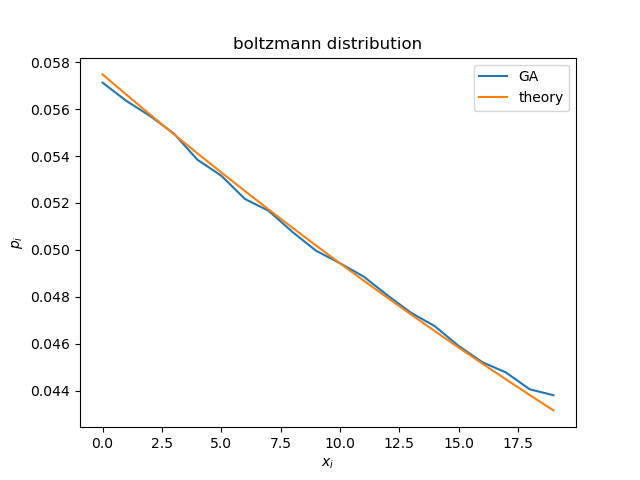
\includegraphics[width=\linewidth, height=0.63\linewidth]{images/boltzmann result.png}
        \caption{볼츠만 분포의 수렴 결과}
        \label{fig:prob1_6_1}
    \end{minipage}
\end{figure}
\begin{figure}[!htb]
    \centering
    \begin{minipage}{.5\textwidth}
        \centering
        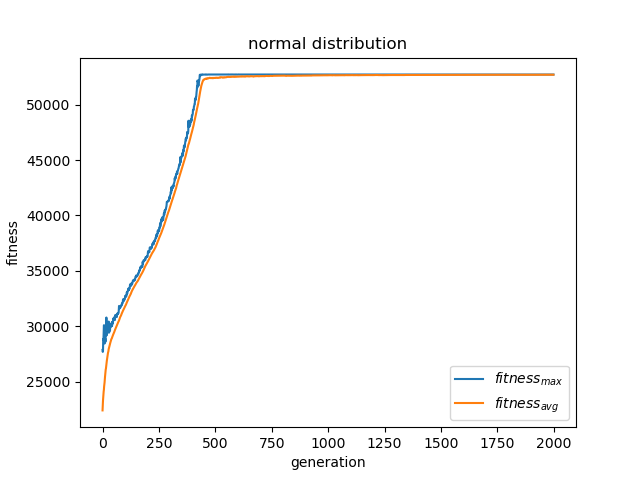
\includegraphics[width=\linewidth, height=0.63\linewidth]{images/normal convergence fitness.png}
        \caption{정규 분포의 적합도 수렴 양상}
        \label{fig:normal fitness}
    \end{minipage}%
    \begin{minipage}{0.5\textwidth}
        \centering
        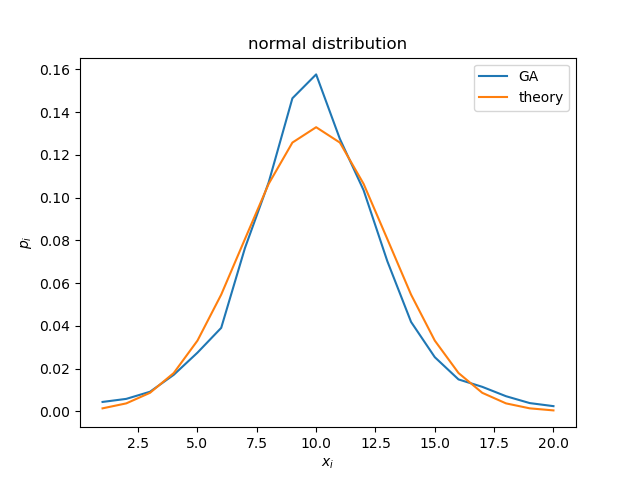
\includegraphics[width=\linewidth, height=0.63\linewidth]{images/normal result.png}
        \caption{정규 분포의 수렴 결과}
        \label{fig:normal result}
    \end{minipage}
\end{figure}